\section{Summarising the Posterior Distribution}
The posterior is too much information. We need to summarise it. This is mostly
because, as mere mortals, we might want to communicate our results as a short,
easily remembered ``sound-bite''. For example, say you were trying to estimate
a parameter, and a colleague asked you to state your uncertainty about the
parameter. Well, your posterior distribution might be complicated, it might
have bumps and wiggles in it, or some other kind of structure.
Figure~\ref{fig:complicated_posterior} shows an example of what a complicated
posterior distribution might look like. If this was your result, your colleague
might not care about all the little wiggles in this plot. They just want to know
the ``big picture'' of your results.
\begin{figure}[h!]
\begin{center}
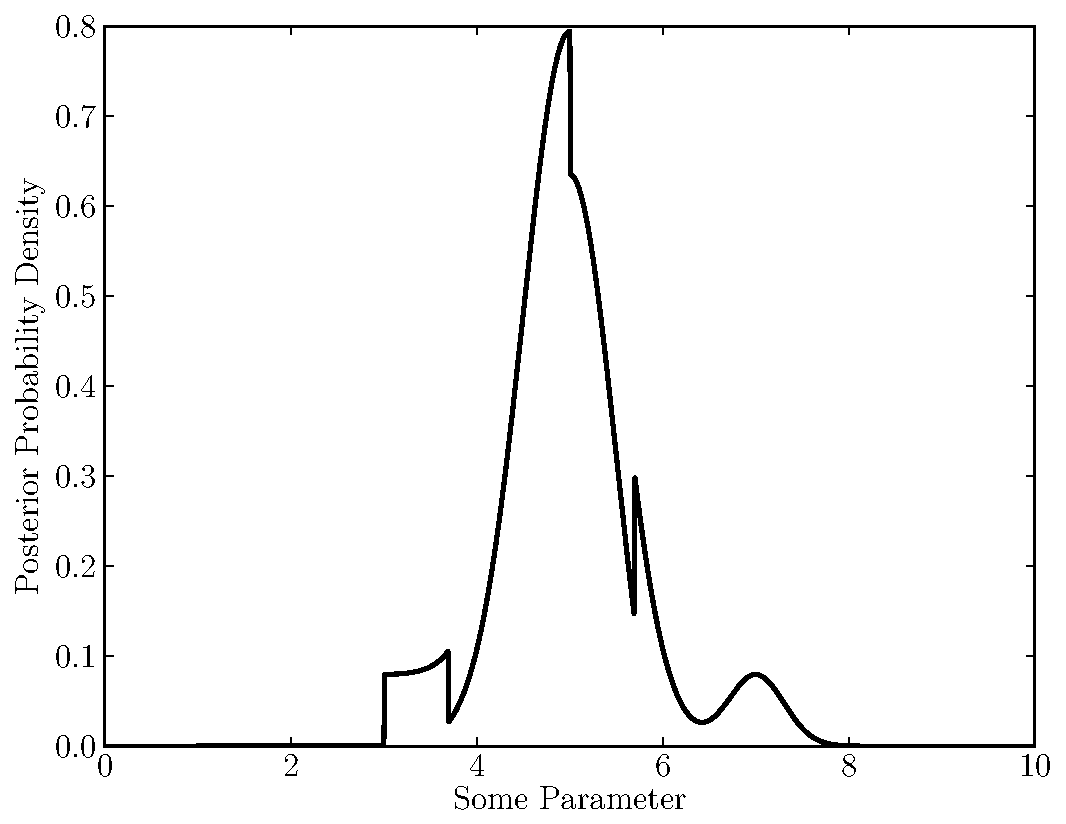
\includegraphics[scale=0.6]{Figures/complicated_posterior.pdf}
\caption{A complicated posterior distribution.\label{fig:complicated_posterior}}
\end{center}
\end{figure}

\begin{framed}
{\bf In descriptive statistics, you often make summaries of a complex data set
(e.g. the mean and the standard deviation) so that you can communicate about
the data set in a concise way. In Bayesian statistics, you often do a similar
thing, but instead of giving a concise description of the data, you give a
concise description of the posterior distribution.}
\end{framed}



\subsection{Point Estimates}


\subsection{Credible Intervals}



